% Especificaciones del tamaño de letra, tamaño de hoja, márgenes, librerias, etc.
\documentclass[12pt, letterpaper]{article}
\usepackage[english]{babel}
\usepackage{fancyhdr}
\usepackage[utf8]{inputenc}
\usepackage[T1]{fontenc}
\usepackage{amsmath}
\usepackage{graphicx}
\usepackage{subcaption}
\usepackage[hidelinks]{hyperref}
\usepackage{url}
\usepackage{amssymb}
\usepackage{float}
\usepackage[margin=1in]{geometry}
\usepackage{listings}
\usepackage{verbatim}
\renewcommand{\baselinestretch}{1.5}

% Enlace Bibliografía
\usepackage{csquotes}
\usepackage[notes,backend=biber]{biblatex-chicago}
\addbibresource{referencias.bib}

% Titulo, autores, fecha.
\title{Práctica \#1: Manipulación de Campos Escalares y Vectoriales}
\author{Carlos A. Vásquez Castañeda \and 1155057 \and Grupo 395}
\date{Febrero 22, 2020}
\pagestyle{fancy}
\fancyhf{}
\rhead{Mecánica de Sustentación}
\lhead{Práctica \#1}
\rfoot{\thepage}


% Inicio del documento
\begin{document}
\maketitle
\section*{Introducción}
Como es costumbre en las ramas de ingeniería, las matemáticas son de gran utilidad para lograr la abstracción de distitnos fenómenos físicos y así poder llegar a modelos que sean fáciles de comprender. El modelado de sistemas físicos como el de los fluidos no es excepción. Si consideramos cada partícula que conforma el fluido estudidado podemos asignarle una posición, componentes de velocidad, de aceleración y otras propiedades físicas de interés. Independientemente de aquello que se quiera modelar, ya es posible contar con una base a partir de esta abstracción del fluido, otorgándonos un vector para cada partícula que represente su estado físico en el espacio. 

En este punto de la abstracción podemos notar que la utilización de la mecánica y cálculo vectorial es de gran ayuda. La introducción de funciones multivariables, campos escalares y campos vectoriales nos permiten tomar cualquier subcojunto del conjunto $\mathbb{R}^n$ y generar una imagen de éste con m-dimensiones, lo cual efectivamente nos otorgaría una aplicación de la forma:
\begin{equation}
	f : D \subset \mathbb{R}^n \rightarrow \mathbb{R}^m
\end{equation}

De esta manera formalizamos la noción de funciones multivariables, donde cada punto $X \in D$ le hace corresponer un único punto $Y \in \mathbb{R}^m$, que  podemos denotar de la forma $Y = f(X)$ y lo llamaremos la \textit{imagen} del punto $X$ mediante la aplicación $f$. Esta aplicación se puede aplicar a cualquier conjunto que sea topológicamente homomorfo a $\mathbb{R}^n$

La ecuación (1) resulta ser la forma de las aplicaciones multivariables más general, y de aquí podemos partir para definir los campos escalares y campos vectoriales.

Un \textbf{campo escalar} es una función real de varias variables en la que a cada punto de su dominio se le asigna el valor que toma una determinada magnitud escalar sobre dicho punto. Expresado de manera análoga a la ecuación (1):

\begin{equation}
	f : D \subset \mathbb{R}^n \rightarrow \mathbb{R}
\end{equation}

La imagen de X es reubicada en la recta de número reales. Por este motivo es que se les llama campos escalares. Podemos iniciar con n-dimensiones pero siempre debemos de obtener un valor concreto dentro de la recta real para que sea considerado un campo escalar.

Por otro lado, un \textbf{campo vectorial} es una función vectorial de varias variables en la que a cada punto de su dominio se le asigna el vector correspondiente a una determinada magnitud vectorial que actúa sobre dicho punto. Formalmente se expresa de la misma manera que la ecuación (1).

Como se decía a inicios de esta sección, estas herramientas resultan útiles para representar partículas con distintas propiedades físicas. Ejemplos de campos escalares pueden ser: densidad, temperatura, altura, etc. Ejemplos de campos vectoriales podrían ser: campos de fuerzas (eléctricos, gravitacionales), campos de velocidades (velocidad de un fluido, movimiento del viento, líneas de corriente). En las siguientes secciones veremos el comportamiento de estos campos y sus gráficas resultantes.

\section*{Procedimiento de la Práctica}

\subsection*{Campo Escalar}
Como primer acercamiento al entorno de Wolfram Mathematica, se declaró una función multivariable la cual regresa un valor numérico, y es representada mediante una gráfica de contornos. La declaración de variables es muy sencilla. Por otro lado, la función para graficar contornos necesita ciertos parámetros. Se necesita especificar el rango de la función de las variables independientes, el tamaño de la imagen, el valor de los contornos que se desea visualizar, los colores y el nombre de los ejes. Cada contorno representa una línea donde el valor de de la función es el mismo. Por lo tanto, si lo visualizamos como una altura, estas líneas representan los puntos en donde la altura es la misma.

\begin{figure}[H]
	\centering
	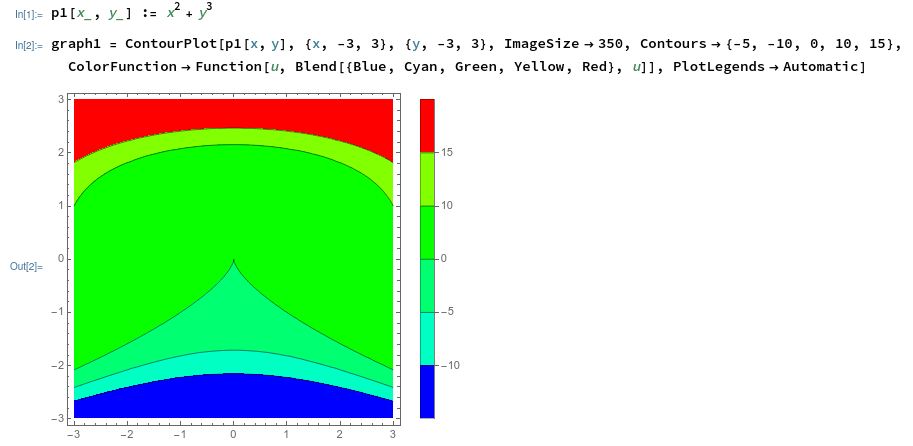
\includegraphics[width=\textwidth]{1.png}
	\caption{Código y gráfica de la función.}
\end{figure}

\subsection*{Campo Vectorial}
Es posible declarar una función vectorial y manipularla al igual que con la función escalar definida anteriormente. La declaración de la función es similar, sin embargo se utilizan corchetes para especificar que se trata de un vector, lo cual se acostumbra en la programación orientada a objetos. De manera similar, esta gráfica se genera mediante la función VectorPLot, la cual toma como parámetros al campo vectorial, los intervalos de las variables independientes y especificaciones de los vectores que se dibujan en pantalla. 

\begin{figure}[H]
	\centering
	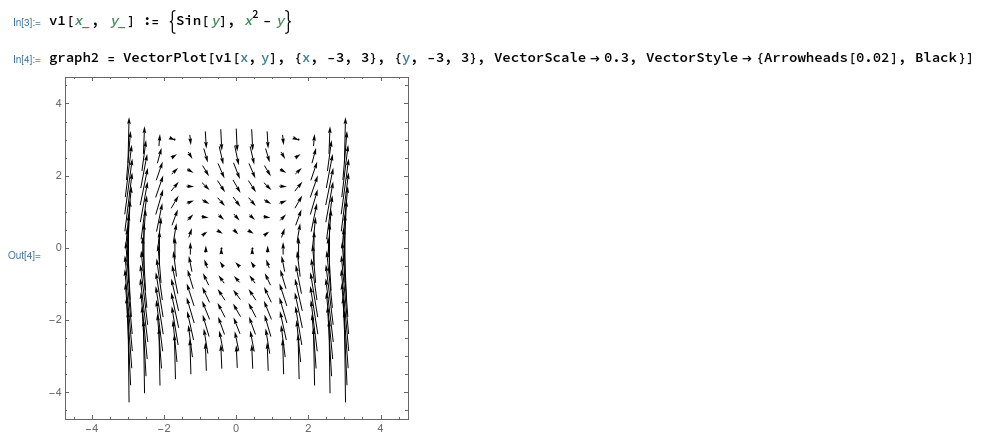
\includegraphics[width=\textwidth]{2.png}
	\caption{Código y gráfica del campo vectorial.}
\end{figure}

También es posible obtener la magnitud de estas funciones mediante la función de norma euclidiana ya integrada en Mathematica.

\begin{figure}[H]
	\centering
	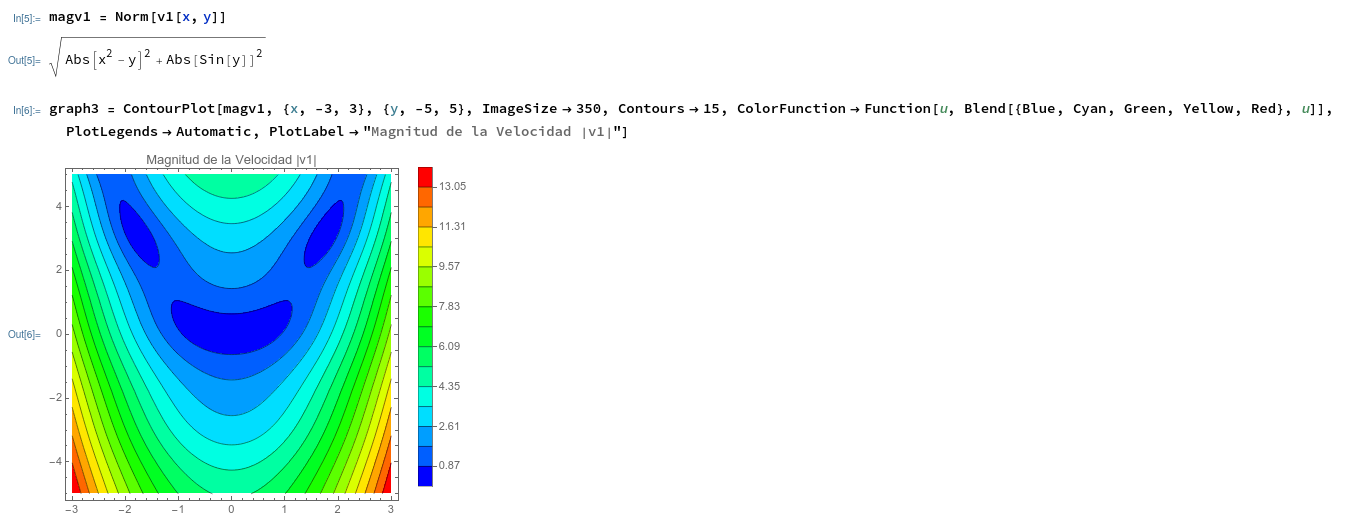
\includegraphics[width=\textwidth]{3.png}
	\caption{Cálculo y representación gráfica de la norma de la función vectorial.}
\end{figure}
\subsection*{Gradiente}
Una vez explorada la declaración de estos distintos tipos de funciones y arreglos, algunas operaciones que es posible hacer con éstos son las de gradiente, divergencia y rotacional. La operación de gradiente se aplica a los campos escalares para hallar la dirección en la cual se halla el cambio más rápido de la función. Es análogo a las derivadas de cálculo de una sola variable.

\begin{figure}[H]
	\centering
	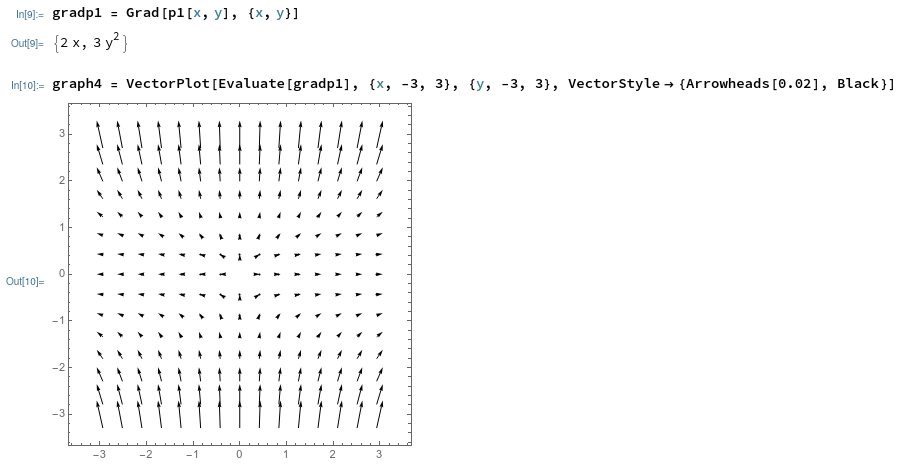
\includegraphics[width=\textwidth]{4.png}
	\caption{Gradiente de la función escalar definida anteriormente.}
\end{figure}

Podemos superponer las gráficas para ver cómo embonan entre ellas
\begin{figure}[H]
	\centering
	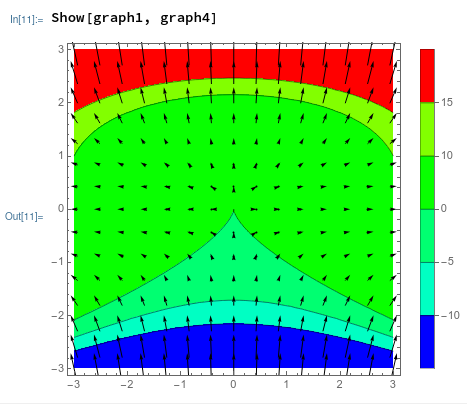
\includegraphics[width=0.5\textwidth]{5.png}
	\caption{Superposición de las gráficas de campo escalar y su gradiente.}
\end{figure}

\subsection*{Divergencia}
Una cantidad de interés para la mecánica de fluidos y de sustentación es la de divergencia. En un campo vectorial es posible medir la diferencia de flujo entrante y saliente de una región dada. Esta operación es la que llamamos divergencia. La sintaxis es bastante similar a la de las otras funciones.

\begin{figure}[H]
	\centering
	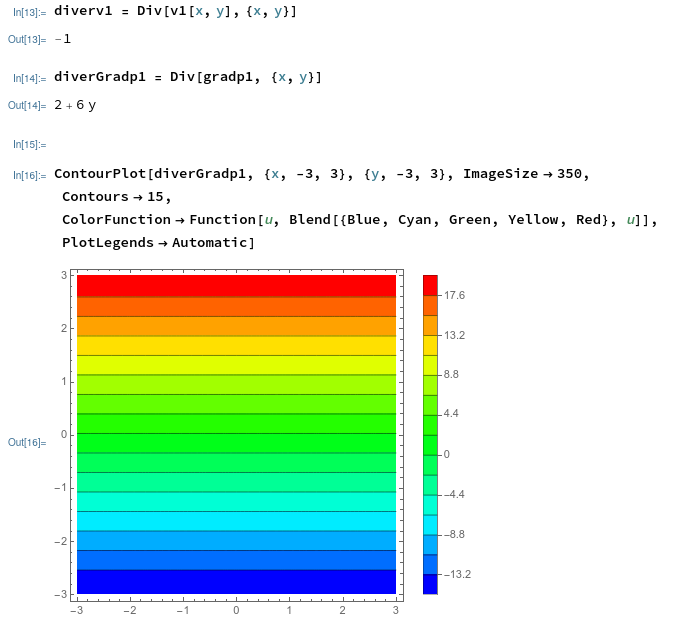
\includegraphics[width=\textwidth]{6.png}
	\caption{Divergencia del campo vectorial y el gradiente de la función escalar.}
\end{figure}

La interpretación es, si la divergencia es menor a 0, se dice que el fluido se comprime, o entra a la región. Y viceversa si la divergencia es mayor a 0.

\subsection*{Campo Vectorial Numérico}
Los campos vectoriales se pueden generar de muchas maneras, la que hemos explorado hasta el momento es mediante la definición de funciones arbitrarias. Sin embargo, en la realidad estos campos vectoriales se modelan mediante la designación de coordenadas a distintos puntos mediante programas de simulación. En éstos podemos modelar objetos y fluidos, los cuales no proporcionarán un campo escalar único con propiedades físicas definidas. Con estos datos podemos calcular distintas propiedades físicas como el campo de velocidades, de mucha utilidad en dinámica de fluidos.

Mediante los archivos proporcionados en clase, hemos importado las coordenadas de los puntos, sus velocidades y presiones. La manipulación de estos datos nos ayudará a visualizar el estado físico del sistema.

\begin{figure}[H]
	\centering
	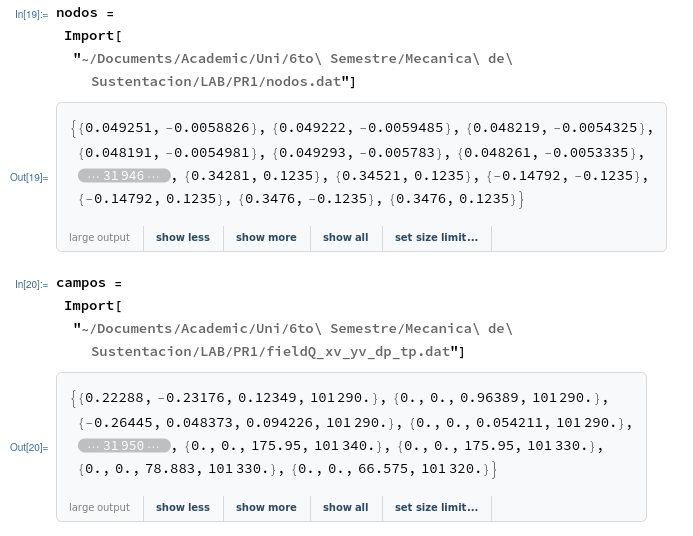
\includegraphics[width=\textwidth]{7.png}
	\caption{Importación de los nodos y datos de los campos vectoriales del perfil alar.}
\end{figure}

Al renderizar estos puntos importados obtendremos la ubicación de los puntos individuales.

\begin{figure}[H]
	\centering
	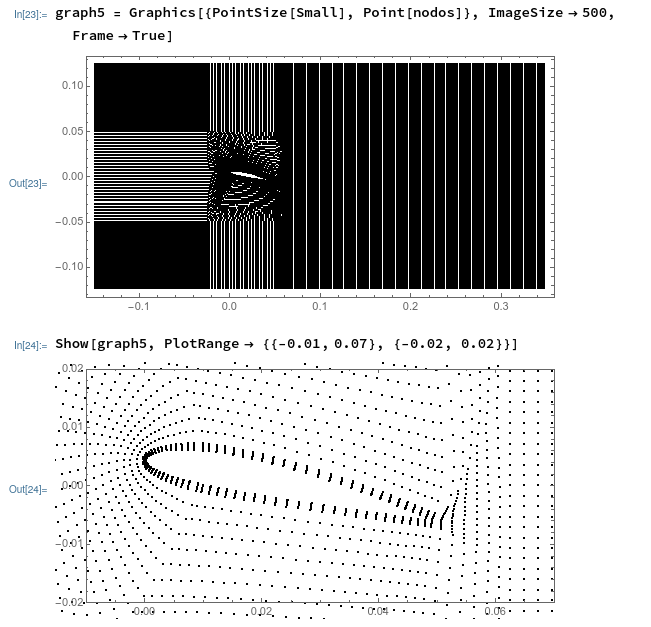
\includegraphics[width=\textwidth]{8.png}
	\caption{Visualización de los puntos.}
\end{figure}

Podemos ver cómo los puntos delinean el contorno del perfil alar, pero esto sólo son los puntos específicos que se utilizaron para la discretización de las líneas que representaban al modelo de perfil alar. A partir de los demás datos importados, podemos mezclarlos para visualizar las distintias propiedades del sistema como lo es la velocidad en la componente direccional $x$.

\begin{figure}[H]
	\centering
	
\includegraphics[width=\textwidth]{9.png}
	\caption{En las primeras líneas del código se almacenan los datos en variables para una referencia sencilla, posteriormente se grafican los puntos y la velocidad en la componente $x$.}
\end{figure}

A pesar de tener esta visualización, resultad difícil discernir los valores máximos y mínimos de la velocidad. Otra opción para representar estos valores es utilizando contornos como en los primeros ejemplos. Para hacer esto y que la gráfica que obtengamos sea reconocible, necesitamos obtener el \textit{aspect ratio} de la región que graficaremos. Esto lo obtendremos mediante los valores de la coordenada X máxima, la mínima y los valores de la coordenada Y máxima y mínima. Se muestra a continuación el bloque de código que se encarga de esto.

\begin{figure}[H]
	\centering
	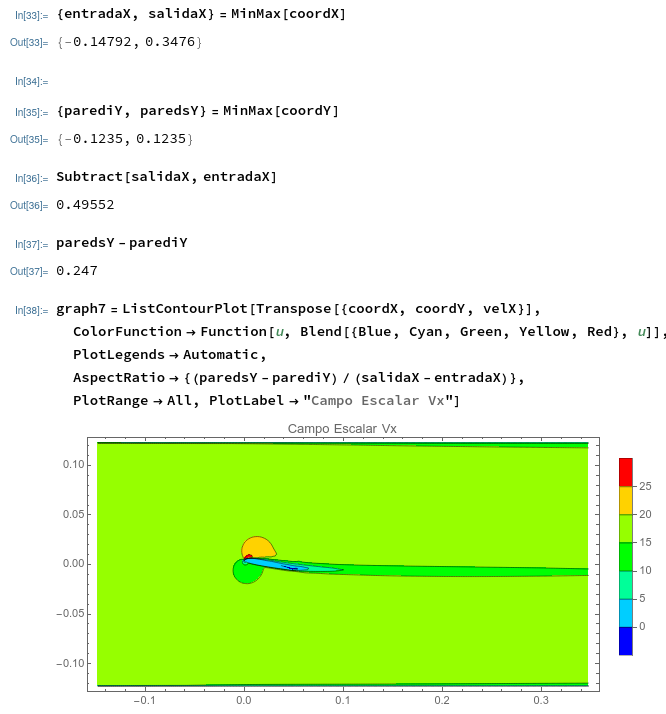
\includegraphics[width=\textwidth]{10.png}
	\caption{Obtención de las coordenadas, el \textit{aspect ratio}, y gráfica de la función en contornos.}
\end{figure}

Aún resulta un poco complejo visualizar en qué punto se encuentra el valor máximo y mínimo de la velocidad en la componente $x$, para esto podemos ordenar al arreglo de número que tenemos de manor a mayor, o viceversa, y extraer el primer punto con sus valores, como se muestra a continuación.

\begin{figure}[H]
	\centering
	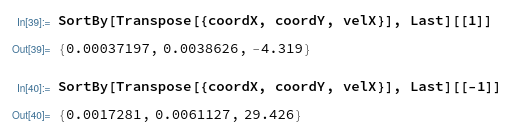
\includegraphics[width=\textwidth]{11.png}
	\caption{Reordenamiento e impresión de los valores máximos y mínimos de la velocidad en la  componente en $x$.}
\end{figure}

Posteriormente, para un mejor análisis de nuestro perfil, es posible generar una superficie, donde se unen los puntos, lo cual nos ayudará aún más a visualizar nuestros datos.

\begin{figure}[H]
	\centering
	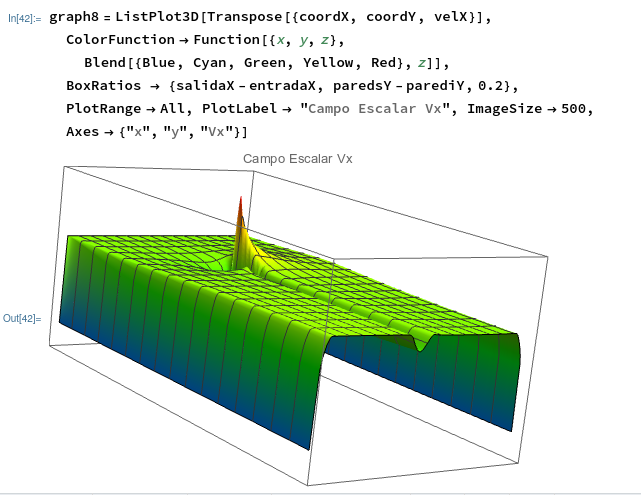
\includegraphics[width=0.8\textwidth]{17.png}
	\caption{Superficie de los datos de perfil alar.}
\end{figure}

Esta gráfica es útil, pero si deseamos ser aún más precisos es conveniente realizar cortes de la gráfica para lograr inspeccionarlos más a fondo. Esto es posible si seleccionamos un rango de valores, digamos valores de la coordenada Y, cuyas abscisas sean una cierta coordenada X establecida. Si deseamos analizar el corte de la entrada del flujo del fluido podemos hacerlo de la siguiente manera.

\begin{figure}[H]
	\centering
	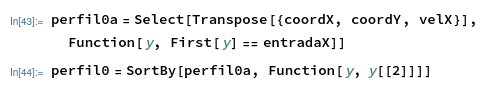
\includegraphics[width=\textwidth]{18.png}
	\caption{Obtención de las coordenadas y su reordenamiento.}
\end{figure}

Esto resultará en la siguiente gráfica.

\begin{figure}[H]
	\centering
	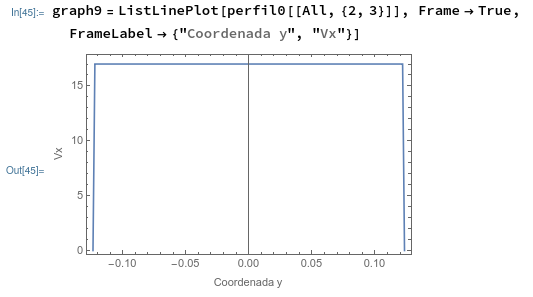
\includegraphics[width=\textwidth]{19.png}
	\caption{Corte de la superficie de la figura 12 en la entrada.}
\end{figure}

Se sigue un procedimiento similar para encontrar el corte de la superficie en la salida del sistema.

\begin{figure}[H]
	\centering
	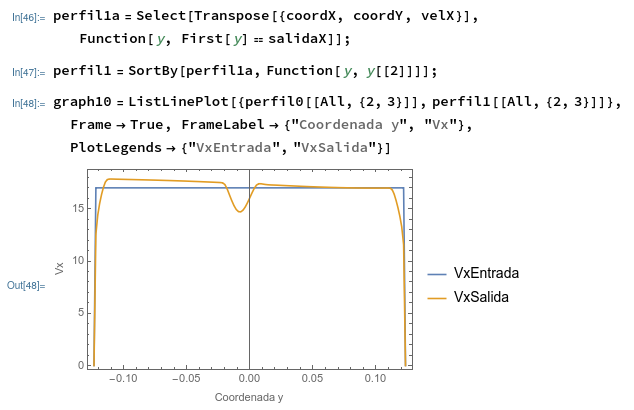
\includegraphics[width=\textwidth]{20.png}
	\caption{Superposición de las gráficas de los cortes hechos de la superficie.}
\end{figure}

Estos dos cortes son de gran utilidad, sin embargo si deseeamos trazar un perfil en un punto específico, digamos, cuando $x = 0$ obtendremos un conjunto vacío de puntos. Esto debido a que la discretización de los puntos del fluido no son exactamente 0 en su componente de posición X. Para encontrar este corte, lo que se deberá de hacer es hallar aquél conjunto de puntos cuyas coordenadas en X se aproximen al cero. Para encontrar esto y visualizarlo procedemos a escribir el siguiente código.

\begin{figure}[H]
	\centering
	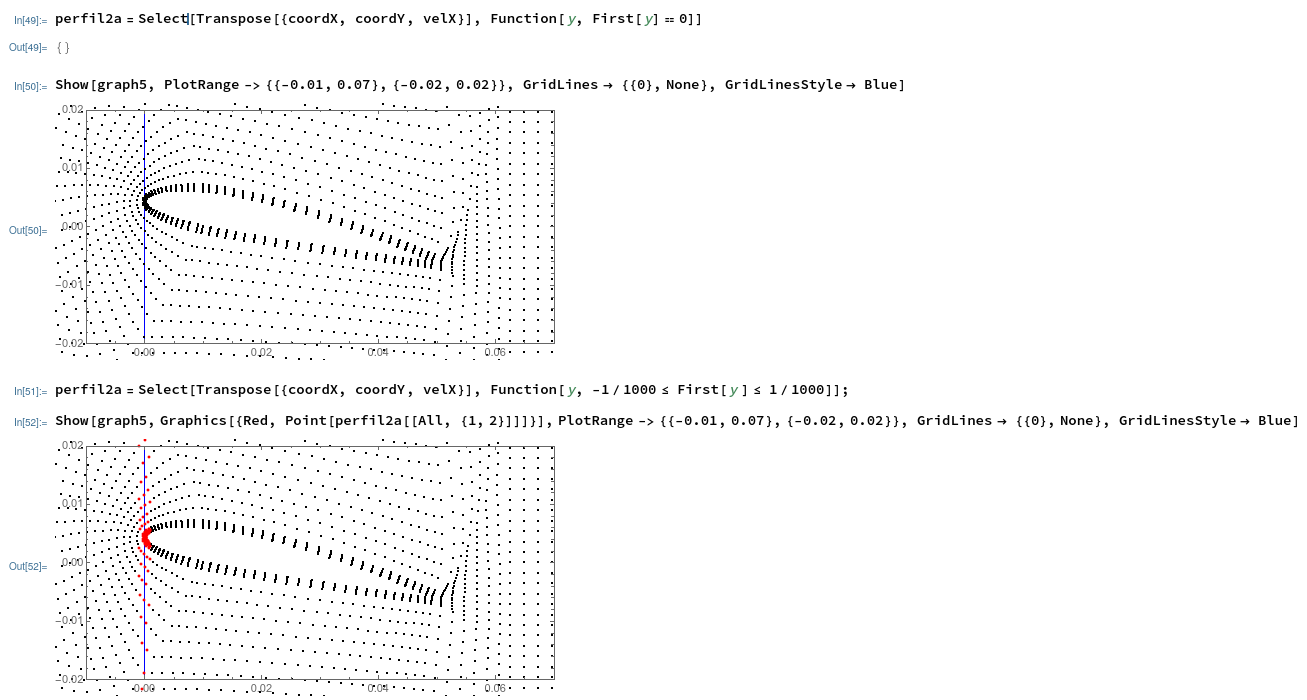
\includegraphics[width=\textwidth]{21.png}
	\caption{Obtención de los puntos que aproximandamente son $x = 0$, así como su visualización.}
\end{figure}

Nótese que se da un rango a los valores de la coordenada X, para así obtener la franja roja mostrada en la figura. Ahora, a partir de estos datos, podemos realizar la superposición de los tres cortes para su análisis posterior.

\begin{figure}[H]
	\centering
	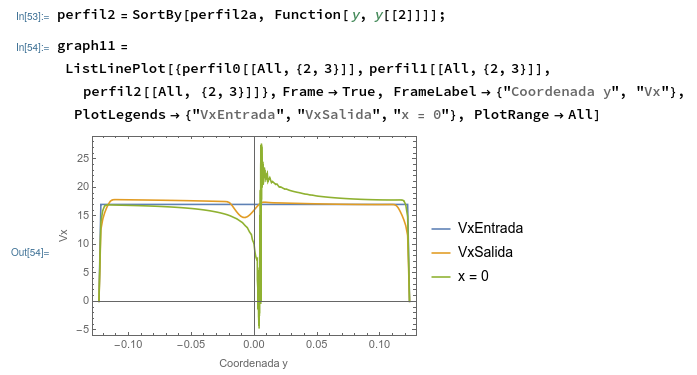
\includegraphics[width=0.8\textwidth]{22.png}
	\caption{Gráficas superpuestas de los distintos cortes creados.}
\end{figure}

Como última forma de visualizar las partículas es mediante la construcción del campo vectorial.

\begin{figure}[H]
	\centering
	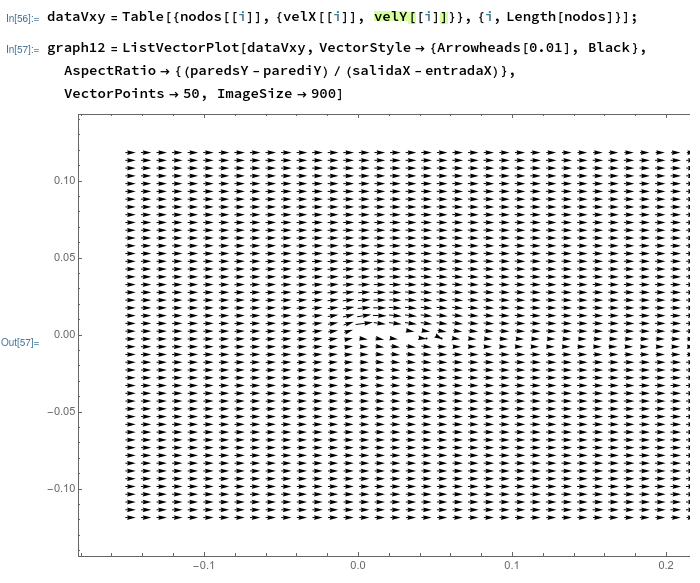
\includegraphics[width=\textwidth]{24.png}
	\caption{Campo vectorial de las partículas del fluido.}
\end{figure}

Si deseamos enfocarnos en el perfil alar es posible realizar un acercamiento.

\begin{figure}[H]
	\centering
	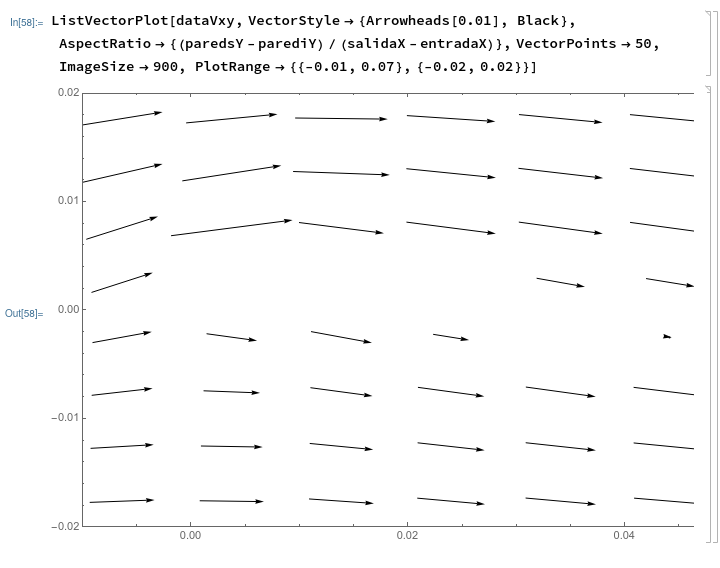
\includegraphics[width=\textwidth]{25.png}
	\caption{Acercamiento del campo vectorial.}
\end{figure}
\section*{Ejercicios}
\begin{enumerate}
	\item Discuta acerca del resultado anterior, ¿es correcto obtener valores de $V_x$ negativos? 

		Pensando en el fenómeno físico, es natural encontrar estos valores. El simple hecho de la creación de vórtices y el choque de las partículas con el perfil alar implican un cambio de dirección en las partículas del fluido, lo cual indicaría que es posible tener estos cambios de velocidad en un sentido negativo y así modificar el movimiento, llevándolo a hacer estructuras como los vórtices al final del perfil alar.

	\item Adicional a $V_x$, obtena para el punto donde sucede la \textbf{máxima} velocidad x de los campos restantes: $V_y$, dp, tp.
	\item Adicional a $V_x$, obtena para el punto donde sucede la \textbf{mínima} velocidad x de los campos restantes: $V_y$, dp, tp.

		Podemos responder el ejercicio \textbf{2 y 3} al mismo tiempo mediane la siguientes líneas de código:

		\begin{figure}[H]
			\centering
			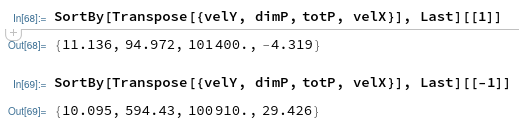
\includegraphics[width=\textwidth]{16.png}
			\caption{Valores de $V_y$, presión dinámica y presión total en los puntos donde $V_x$ es máxima y mínima, respectivamente.}
		\end{figure}

	\item Obtenga las representaciones gráficas o trazos de los campos escalares restantes: $V_y$, dp, tp.
	\item Calcule los valores máximos y mínimos de los campos restantes, así como las coordenadas de los puntos donde suceden.

		\textbf{Los ejercicios 4 y 5} es posible contestarlos ambos al mismo tiempo. A continuación se muestran los resultados.

		\begin{figure}[H]
			\centering
			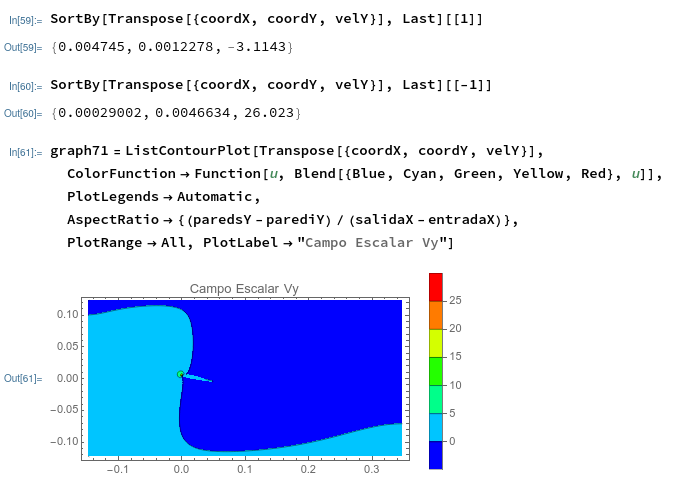
\includegraphics[width=0.7\textwidth]{12.png}
			\caption{$V_y$}
		\end{figure}

		\begin{figure}[H]
			\centering
			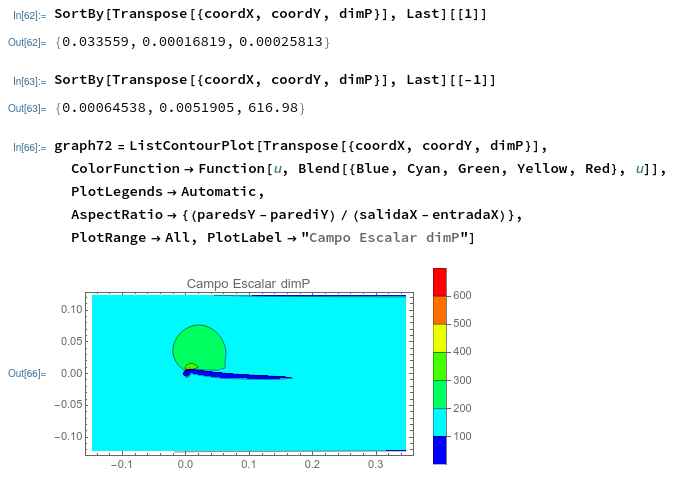
\includegraphics[width=0.7\textwidth]{13.png}
			\caption{Presión dinámica.}
		\end{figure}

		\begin{figure}[H]
			\centering
			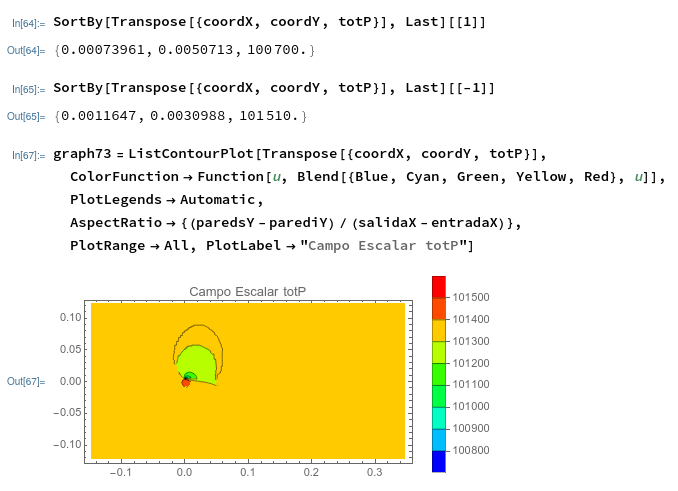
\includegraphics[width=0.7\textwidth]{14.png}
			\caption{Presión total.}
		\end{figure}

		Así como se hizo en la figura 10 y 11, se realizó el mismo procedimiento pero esta vez utilizando los datos de las distintas cantidades físicas con las que se contaban. 
	\item Discuta sobre los resultados obtenidos en el campo escalar $V_y$.

		La gráfica muestra mayormente una variación en los puntos que están al inicio del perfil alar. Debido a la geometría del perfil, es razonable que las partículas tengan un aumento en su componente de velocidad vertical. Es por eso que estas partículas cercanas presentan mayor velocidad vertical en este punto, sin embargo, las demás partíciulas del fluido a su alrededor cambian sus trayectorias, normalizándolas y dándoles una dirección similar a las del fluido en general, la cual es casi puramente horizontal. En otras palabras, la ausencia de componente vertical en la velocidad es bastante grande debido a la dirección del flujo que se eligió.
		\begin{figure}[H]
			\centering
			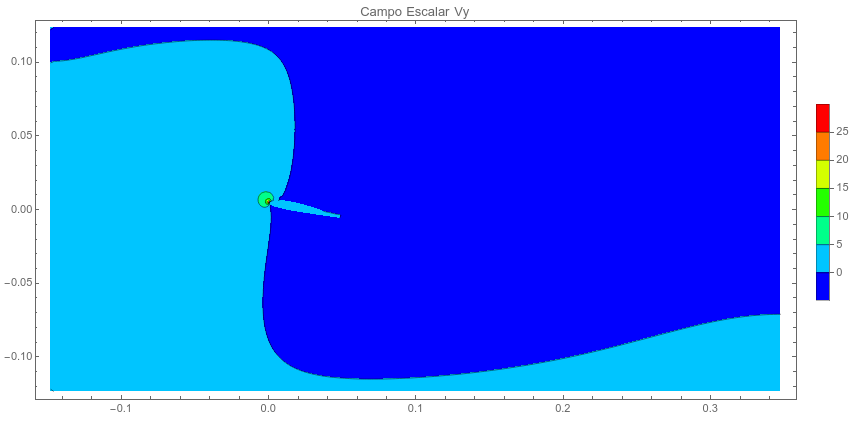
\includegraphics[width=\textwidth]{15.png}
			\caption{Detalle de la gráfica de contorno para $V_y$.}
		\end{figure}
	\item Trace los perfiles $V_y$ para las mismas localizaciones (entrada, salida y $x = 0$).
		
		\begin{figure}[H]
			\centering
			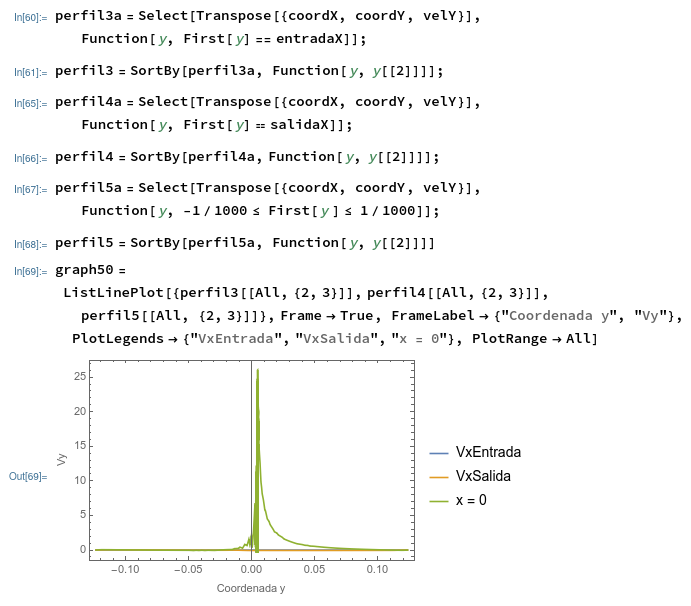
\includegraphics[width=0.7\textwidth]{23.png}
			\caption{Cortes para $V_y$.}
		\end{figure}

	\item Trace los perfiles $|V|$ para las mismas localizaciones (entrada, salida y $x = 0$).

		\textit{Esta pregunta no supe cömo llegar a la norma de ambas magnitudes porque se encontraban en arreglos distintos ($V_x$ y $V_y$).}
	\item Discuta sobre los perfiles de velocidad, ¿cuál es el efecto de la obstrucción del perfil alar sobre éstos?

		Aumenta dramáticamente la velocidad en ambas componentes de la velocidad.
	\item Comente cuál es el comportamiento de la velocidad en las paredes y su cercanía.

		La velocidad es efectivamente cero, y eso es algo que hemos de esperar de estas simulaciones ya que hemos definido como condición de frontera esta particularidad.

\end{enumerate}

\section*{Conclusión}
A partir de los resultados obtenidos mediante el programa Mathematica, es sencillo ver cómo los resultados necesitan de interpretación después de haber llegado a estos campos vectoriales. Estas herramientas proporcionadas por Mathematica nos permiten realizar estas intepretaciones de manera mucho más simple. La versatilidad de las funciones y el modo en el que se modifican los arreglos y datos resulta muy amigable para llegar a la toma de decisiones adecuada.

La utilización de las distintas operaciones vectoriales son utilizadas con mucha frecuencia, en especial en la mecánica de sustentación y esto puede hacer la diferencia entre un perfil alar que sea altamente fiable a uno que sea inestable.

%%%%%  Bib
\renewcommand\refname{References}
\printbibliography
\end{document}
